\documentclass[]{article}
\usepackage{lmodern}
\usepackage{amssymb,amsmath}
\usepackage{ifxetex,ifluatex}
\usepackage{fixltx2e} % provides \textsubscript
\ifnum 0\ifxetex 1\fi\ifluatex 1\fi=0 % if pdftex
  \usepackage[T1]{fontenc}
  \usepackage[utf8]{inputenc}
\else % if luatex or xelatex
  \ifxetex
    \usepackage{mathspec}
  \else
    \usepackage{fontspec}
  \fi
  \defaultfontfeatures{Ligatures=TeX,Scale=MatchLowercase}
\fi
% use upquote if available, for straight quotes in verbatim environments
\IfFileExists{upquote.sty}{\usepackage{upquote}}{}
% use microtype if available
\IfFileExists{microtype.sty}{%
\usepackage{microtype}
\UseMicrotypeSet[protrusion]{basicmath} % disable protrusion for tt fonts
}{}
\usepackage[margin=1in]{geometry}
\usepackage{hyperref}
\hypersetup{unicode=true,
            pdftitle={literature},
            pdfauthor={Masumbuko Semba},
            pdfborder={0 0 0},
            breaklinks=true}
\urlstyle{same}  % don't use monospace font for urls
\usepackage{longtable,booktabs}
\usepackage{graphicx,grffile}
\makeatletter
\def\maxwidth{\ifdim\Gin@nat@width>\linewidth\linewidth\else\Gin@nat@width\fi}
\def\maxheight{\ifdim\Gin@nat@height>\textheight\textheight\else\Gin@nat@height\fi}
\makeatother
% Scale images if necessary, so that they will not overflow the page
% margins by default, and it is still possible to overwrite the defaults
% using explicit options in \includegraphics[width, height, ...]{}
\setkeys{Gin}{width=\maxwidth,height=\maxheight,keepaspectratio}
\IfFileExists{parskip.sty}{%
\usepackage{parskip}
}{% else
\setlength{\parindent}{0pt}
\setlength{\parskip}{6pt plus 2pt minus 1pt}
}
\setlength{\emergencystretch}{3em}  % prevent overfull lines
\providecommand{\tightlist}{%
  \setlength{\itemsep}{0pt}\setlength{\parskip}{0pt}}
\setcounter{secnumdepth}{5}
% Redefines (sub)paragraphs to behave more like sections
\ifx\paragraph\undefined\else
\let\oldparagraph\paragraph
\renewcommand{\paragraph}[1]{\oldparagraph{#1}\mbox{}}
\fi
\ifx\subparagraph\undefined\else
\let\oldsubparagraph\subparagraph
\renewcommand{\subparagraph}[1]{\oldsubparagraph{#1}\mbox{}}
\fi

%%% Use protect on footnotes to avoid problems with footnotes in titles
\let\rmarkdownfootnote\footnote%
\def\footnote{\protect\rmarkdownfootnote}

%%% Change title format to be more compact
\usepackage{titling}

% Create subtitle command for use in maketitle
\newcommand{\subtitle}[1]{
  \posttitle{
    \begin{center}\large#1\end{center}
    }
}

\setlength{\droptitle}{-2em}

  \title{literature}
    \pretitle{\vspace{\droptitle}\centering\huge}
  \posttitle{\par}
    \author{Masumbuko Semba}
    \preauthor{\centering\large\emph}
  \postauthor{\par}
      \predate{\centering\large\emph}
  \postdate{\par}
    \date{December 6, 2018}

\usepackage{booktabs}
\usepackage{longtable}
\usepackage{array}
\usepackage{multirow}
\usepackage[table]{xcolor}
\usepackage{wrapfig}
\usepackage{float}
\usepackage{colortbl}
\usepackage{pdflscape}
\usepackage{tabu}
\usepackage{threeparttable}
\usepackage{threeparttablex}
\usepackage[normalem]{ulem}
\usepackage{makecell}

\begin{document}
\maketitle

{
\setcounter{tocdepth}{2}
\tableofcontents
}
\section{Results}\label{results}

\begin{verbatim}
Reading layer `miamba_topology_clean_updated_added_mafia' from data source `e:\Data Manipulation\mafia_kilwa_octopus_mapping\shapefiles\miamba_topology_clean_updated_added_mafia.shp' using driver `ESRI Shapefile'
Simple feature collection with 108 features and 4 fields
geometry type:  MULTIPOLYGON
dimension:      XY
bbox:           xmin: 39.3 ymin: -8.65 xmax: 39.8 ymax: -7.82
epsg (SRID):    4326
proj4string:    +proj=longlat +datum=WGS84 +no_defs
\end{verbatim}

\subsection{Jibondo}\label{jibondo}

Figure \ref{fig:fig-jibondo} is map showing the distribution of outer
and inner coral reefs areas that octopus fisher use as fishing ground at
Jibondo Island in Mafia Island.

\begin{figure}
\centering
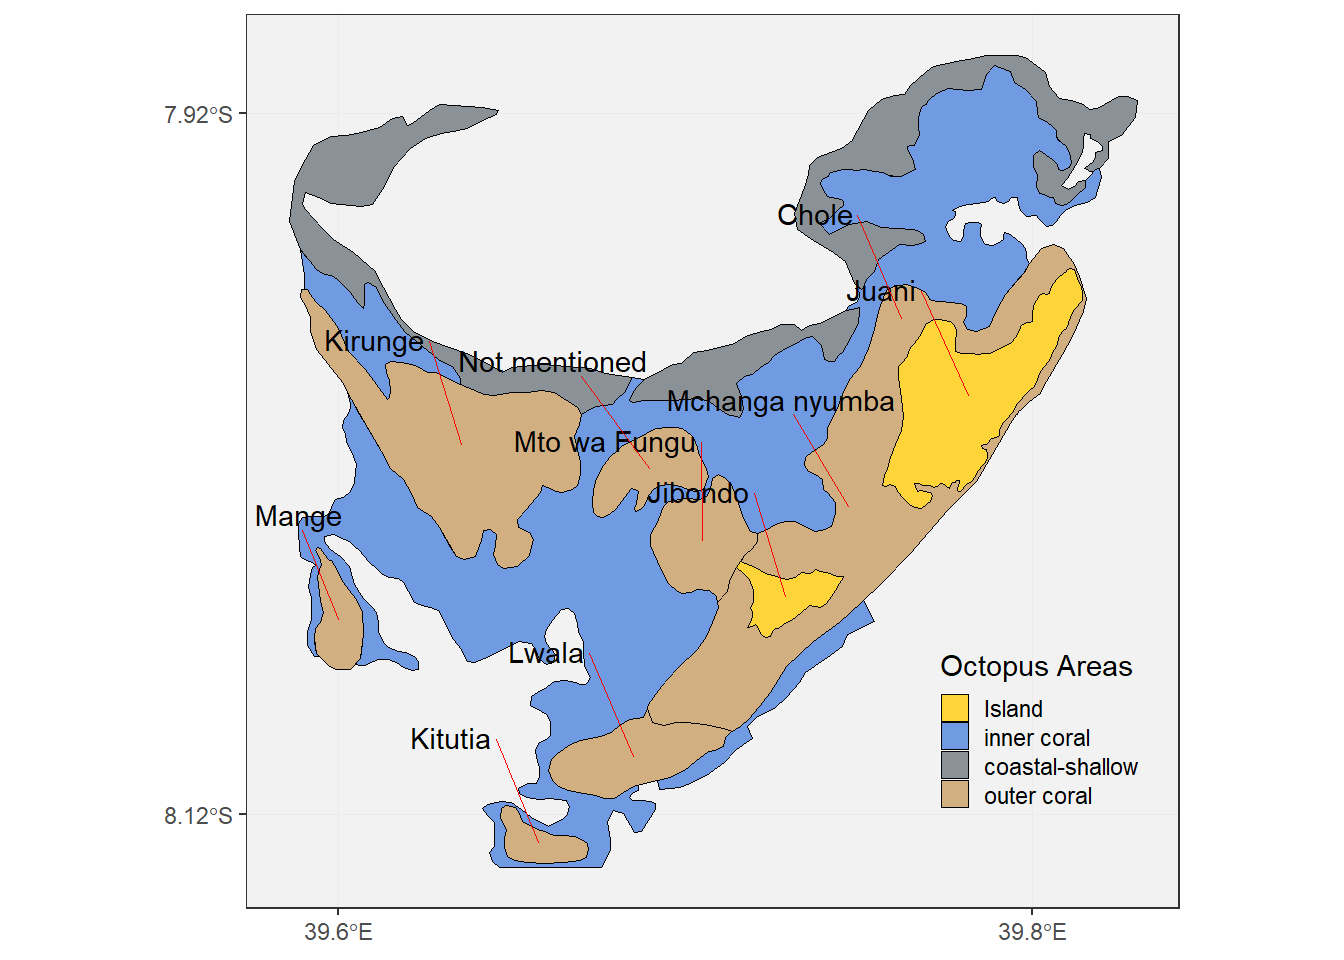
\includegraphics{Results_files/figure-latex/map-jibondo-1.pdf}
\caption{\label{fig:map-jibondo}Coral reef octopus fishing areas used by
fishermen from Jibondo Island}
\end{figure}

\label{tab:tab11}Coral reefs that are mostly used for octopus fishery as
fishing ground in Jibondo Island

Octopus fishery

Fishing ground

Number

Percentage

Mto Mkuu

146

58.167

Jibondo Kusini

65

25.896

Dongo

35

13.944

Kitutia

3

1.195

Chole Bay General Use Zone

1

0.398

Jibondo

1

0.398

Athough the Chole Bay Genera Use Zone appear on the table
\ref{tab:tab11}, it was dropped on the figure \ref{fig:fig-jibondo}
because it is out of the area of focus

\begin{figure}

{\centering 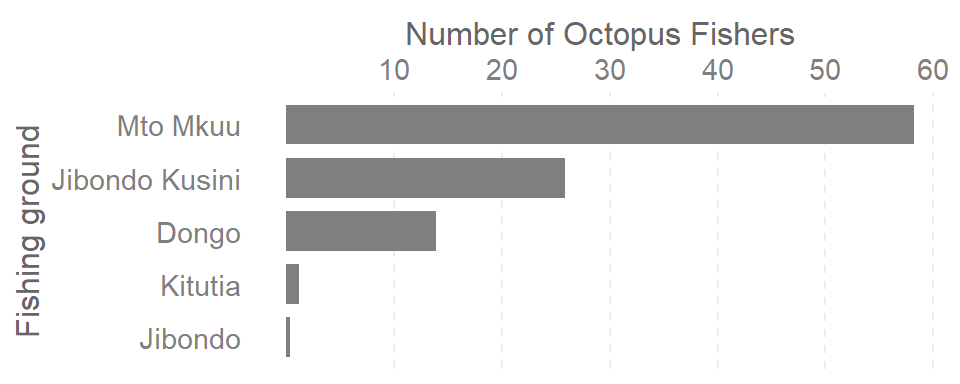
\includegraphics{Results_files/figure-latex/fig-jibondo-1} 

}

\caption{Percentage of octopus fishers at different coral reefs grounds at Jibondo Island}\label{fig:fig-jibondo}
\end{figure}

\subsection{Bwejuu}\label{bwejuu}

Figure \ref{fig:fig-bwejuu} is map showing the distribution of outer and
inner coral reefs areas that octopus fisher use as fishing ground at
Bwejuu Island in Mafia Island. the inner reefs are mostly used by divers
while the outer reefs are mostly exposed during hight tide and
extensively used by both walking and diving octopus fishers

\begin{figure}
\centering
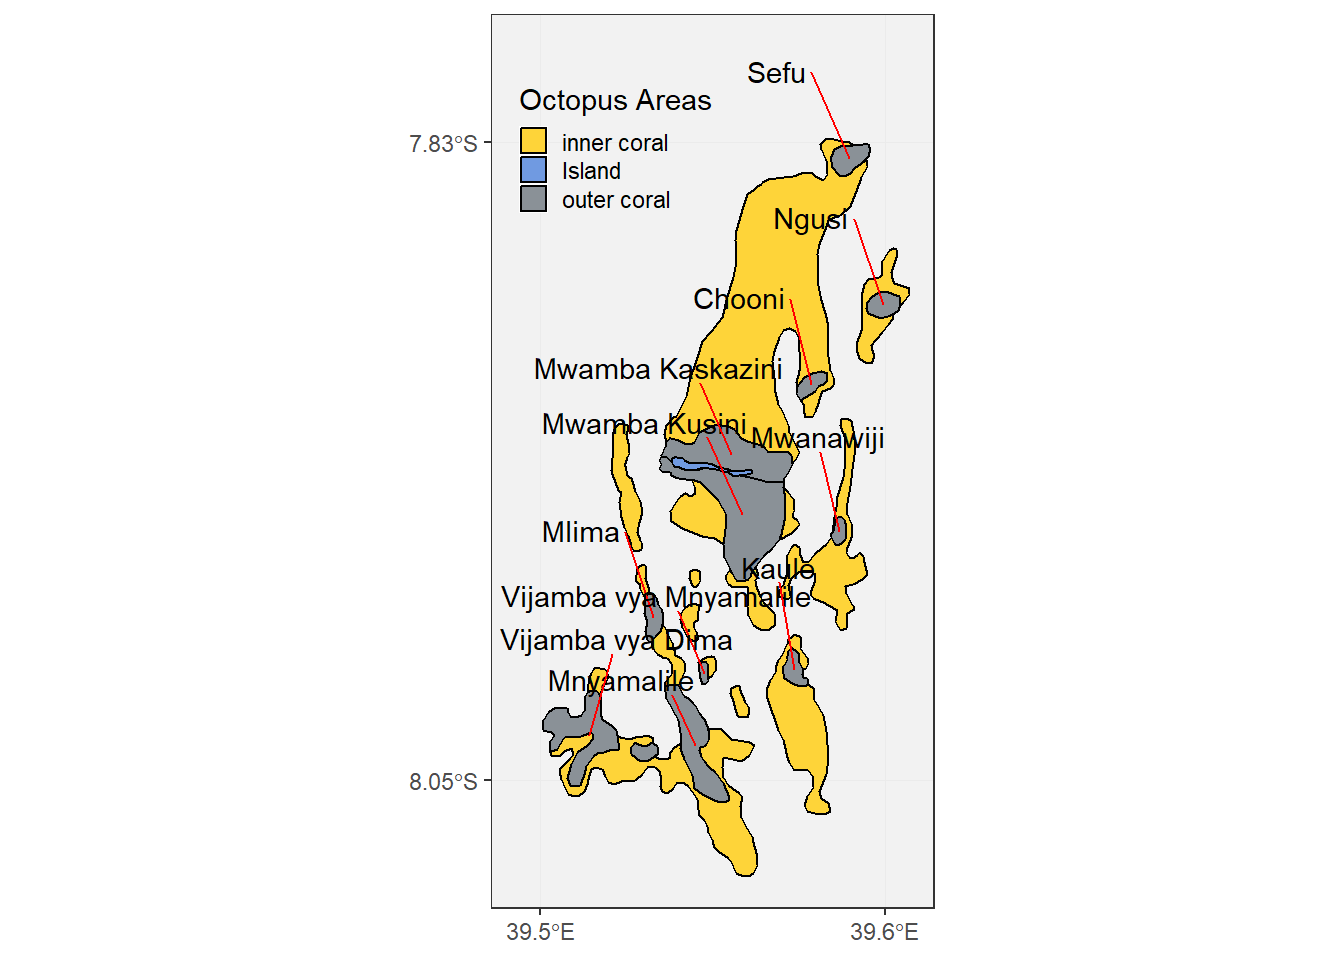
\includegraphics{Results_files/figure-latex/map-bwejuu-1.pdf}
\caption{\label{fig:map-bwejuu}Coral reef octopus fishing areas used by
fishermen from Bwejuu Island}
\end{figure}

\label{tab:tab12}Coral reefs that are mostly used for octopus fishery as
fishing ground in Bwejuu Island

Octopus fishers

Fishing ground

Number

Percentage

Nyamalile

27

57.45

Banda Mrima

8

17.02

Vijambani

4

8.51

Bwejuu Kusini

2

4.25

Kaule

2

4.25

Mwamba Wa Pwani

2

4.25

Mbakare

1

2.13

Ngusi

1

2.13

\begin{figure}

{\centering 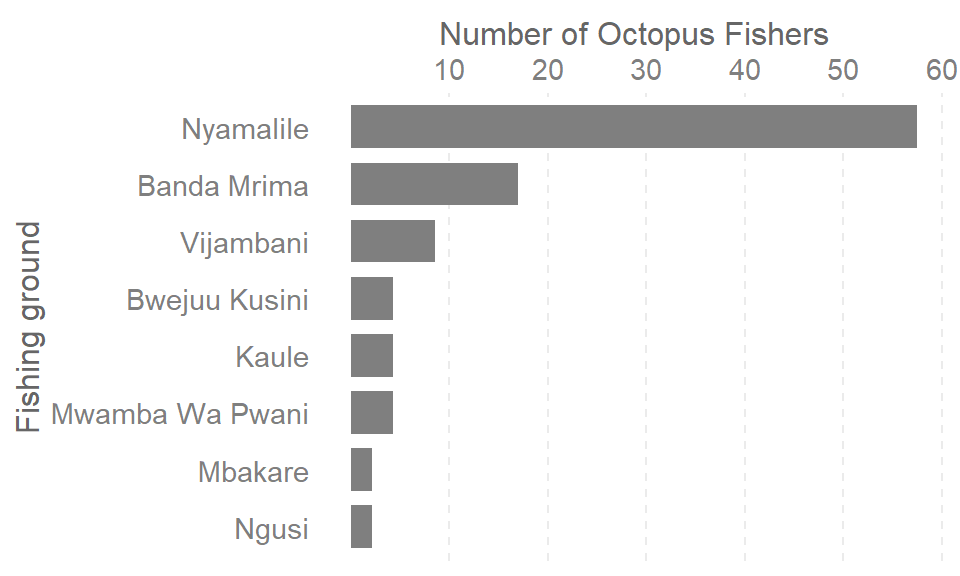
\includegraphics{Results_files/figure-latex/fig-bwejuu-1} 

}

\caption{Percentage of octopus fishers at different coral reefs grounds at Bwejuu Island}\label{fig:fig-bwejuu}
\end{figure}

Figure \ref{fig:cpue-boxplot} show the Octopus fishers from those study
areas located far from human influence (Songosongo and Bwejuu) obtained
relatively higher catch than those close to human activities (Jibondo
and Somanga). In general, octopus fisher at Songosongo and Bwejuu
catches twice as compared to fishers and Jibond and Somanga (Table
\ref{tab:tab12a})

\begin{figure}

{\centering 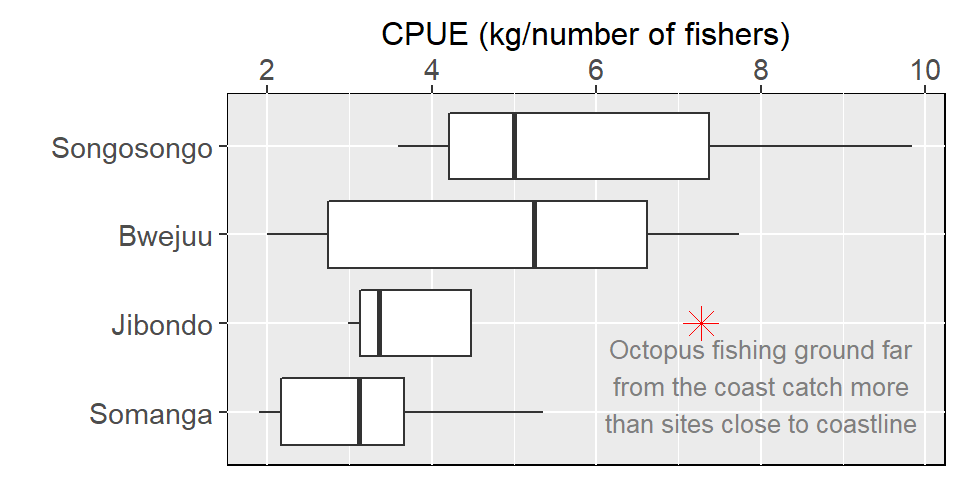
\includegraphics{Results_files/figure-latex/cpue-boxplot-1} 

}

\caption{Catch rate of Octopus for the four study areas}\label{fig:cpue-boxplot}
\end{figure}

\label{tab:tab12a}Frequency and catch rate of octopus fishers

Catch rate (Kg/fishers)

Site

n

CPUE

Error

Jibondo

251

3.27

0.151

Somanga

96

3.29

0.352

Songosongo

68

6.04

0.514

Bwejuu

47

6.44

0.722

\begin{table}[H]
\centering\rowcolors{2}{gray!6}{white}

\begin{tabular}{lrrr}
\hiderowcolors
\toprule
village & count & cpue.bar & cpue.sd\\
\midrule
\showrowcolors
Jibondo & 251 & 3.27 & 0.151\\
Somanga & 96 & 3.29 & 0.352\\
Songosongo & 68 & 6.04 & 0.514\\
Bwejuu & 47 & 6.44 & 0.722\\
\bottomrule
\end{tabular}
\rowcolors{2}{white}{white}
\end{table}


\end{document}
